\documentclass[11 pt]{scrartcl}
\usepackage[header, margin, koma]{tyler}
\usetikzlibrary{automata,arrows,positioning,calc}

\pagestyle{fancy}
\fancyhf{}
\fancyhead[l]{EECS 126 Notes}
\fancyhead[r]{Tyler Zhu}
\cfoot{\thepage}

\begin{document} 
\title{\Large EECS 126 Notes}
\author{\large Tyler Zhu}
\date{\large\today}

\maketitle 

These are course notes for the Spring 2019 rendition of EECS 126, Probability Theory and Random Processes, taught by Professor Kannan Ramchandran. I began these notes five lectures in, but the missing material is mostly CS 70 level probability. Special thanks to Evan Chen, whose .sty file never fails to impress, which is why I've stolen bits of it for these notes.  

\tableofcontents 

\newpage

%TODO: add in a cheat sheet of common formulas, distributions, etc. as we learn them. 

\section{Thursday, February 7th}
\subsection{Announcements}
Couple of announcements. 
\begin{itemize}
    \ii HW 3 is due next Wednesday. 
    \ii Lab 2 is due on Friday. 
    \ii Self grades for both HW and Lab due on Monday. 
    \ii Readings are B\&T, Ch. 3, 4.1-3 and 4.6 
\end{itemize}

\subsection{Mins and Maxes of Exponentials}
We saw already that the exponential random variable has pdf $f_T(t) = \la e^{-\la t}$, and has $\EE[T] = 1/\la$ and $var(T) = 1/\la^2$. 

We also saw how $\min(T_1, T_2, \dots, T_n) \sim \Expo(\la_1+\la_2 + \dots + \la_n)$ for independent exponential variables $T_1, T_2, \dots, T_n$. The key idea used was the memoryless property. 

One example is if we have a hundred lightbulbs that burn out in time proportional to $\Expo(1)$. Then what is the expected time it would take for the first lightbulb to burn out? Of course, this would be $1/100$ since the min is modeled by $\Expo(100)$. 

But what about the maximum? If we have $n$ i.i.d. $\Expo(1)$ random variables $T_i$, what is $\EE[\max(T_1, \dots, T_n)]$? Continuing our previous analogy, we can think of this as asking what the expected time for the last lightbulb to burn out is. 

There's a way to leverage what we've already calculated to do this calculation however! Since the exponential r.v. is memoryless, once the first bulb burns out, we have the same situation again, but with $n-1$ bulbs instead. Hence,   
\[ \EE[\text{time for }n\text{ bulbs to b.o.}] = \EE[\text{1st bulb to b.o.}] + \EE[n-1\text{ remaining bulbs to b.o.}]\]

If we let $S_n$ be the r.v. counting the time it takes for $n$ bulbs to burn out (and using the fact that $\EE[S_1] = 1$), we can rewrite this as 
\begin{align*}
    \EE[S_n] &= \dfrac{1}{n} + \EE[S_{n-1}] \\ 
             &= \dfrac{1}{n} + \dfrac{1}{n-1} + \EE[S_{n-1}] \\ 
             &= \sum_{k=1}^n \dfrac{1}{k} = H_n \approx \ln n + \gamma 
\end{align*}
where $\gamma$ is the Euler-Mascheroni constant. 

Another quick remark: Geometric variables are just discretizations of exponential random variables. (See book). 

Here's a teaser to cap off this section. Suppose you are in line at a post office, and ahead of you two people are waiting to be served with probability $\Expo(1)$ each. Once one of the two are served, you take their place waiting to be served. What is the probability you will be served before the other person? Answer is $1/2$ thanks to the memoryless property. 

\subsection{Standard Normal Distributions}
\begin{definition}
    The PDF of the \emph{standard normal} distribution $\Nor(0,1)$, i.e. with mean $0$ and variance $1$, is 
    \[ f_X(x) \propto e^{-x^2/2} \quad \text{ for } -\infty < x < \infty.\] 
    This is a probability distribution for an appropriate choice of $c$ for which $c\int_{-\infty}^\infty e^{-x^2/2}dx = 1$. 
\end{definition}

You can probably convince yourself that this integral converges, but it's another question to figure out exactly \emph{what} it converges to! 

    To do this, we'll introduce a variable $\alpha$ (effectively computing a more \emph{general} integral) and consider the integral 
    \[ I = \int_{-\infty}^\infty e^{-\alpha x^2/2}dx.\] 
    Then the trick is to consider $I^2$, since we get 
    \[ I^2 = \int_{\RR} e^{-\alpha x^2/2} dx \int_{\RR} e^{-\alpha y^2/2} dy  = \int_{-\infty}^\infty \int_{-\infty}^\infty e^{-\alpha (x^2+y^2)/2}dxdy. \] 
    This should remind you of polar coordinates, where $x^2+y^2 = r^2$ represents the radius. Hence, we will change our variables to achieve that, using 
    \begin{align*} 
        x^2 + y^2 &= r^2 \\ 
        dx\, dy &= r\, dr\, d\theta 
    \end{align*}
    (you can get these by computing the Jacobian (ew)). Substituting gives 
\begin{align*} 
    I^2 &= \int_0^{2\pi}\int_0^{\infty} e^{-\alpha r^2/2} r dr d\theta = 2\pi\int_0^\infty re^{-\alpha r^2} dr  \\ 
        &= (2\pi) \left(-\dfrac{1}{\alpha}e^{-\alpha r^2/2}\right) \Big|^{\infty}_0 = \dfrac{2\pi}{\alpha} 
\end{align*}
    Finally, to get our desired integral, we set $\alpha = 1$ so that $I^2 = 2\pi$ and hence, $I = \sqrt{2\pi}$. This means our PDF is actually 
    \[ f_X(x) = \dfrac{1}{\sqrt{2\pi}} e^{-x^2/2}.\] 

    Let's verify that the mean and variance of this PDF are indeed $0$ and $1$. We know by symmetry about 0 that $\EE[X] = 0$. For the variance, our calculations are simplified because of this, so 
    \[ \Var(X) = \EE[X^2] - \EE[X]^2 = \EE[X^2] = \dfrac{1}{\sqrt{2\pi}}\int_{-\infty}^{\infty} x^2 e^{-\alpha x^2/2} dx.\]
    Now we'll employ differentiation under the integral, which states that if we have some function $f(x,\alpha)$, then 
    \[ \int_a^b \dfrac{\partial}{\partial \alpha} f(x,\alpha) dx = \dfrac{d}{d\alpha}\int_a^b f(x,\alpha) dx.\] 
    We have an integral of the form on the left side, and our goal will be to get to the right side. This means we solve for $f$ to get
    \[ \dfrac{\partial}{\partial \alpha} f(x,\alpha) = x^2e^{-\alpha x^2/2} \implies f(x,\alpha) = -2e^{-\alpha x^2/2}\]
    and plugging this in gives 
    \[ \Var(X) = \dfrac{1}{\sqrt{2\pi}} \dfrac{d}{d\alpha}\int_{\infty}^\infty -2e^{-\alpha x^2/2}dx.\] 
    But we already know this integral! It's the one we just calculated, $I$, which we know is $\sqrt{\frac{2\pi}{\alpha}}$. So we can just substitute this back in to get 
    \[ \Var(X) = -2 \dfrac{d}{d\alpha} \dfrac{1}{\sqrt{\alpha}} = \alpha^{-3/2}. \]
    Our goal is when $\alpha = 1$, which gives us $\Var(X) = 1$ as desired. 

\subsection{Applications of the Standard Normal}
    Sometimes we're interested in integrating the PDF only over certain intervals; this is the CDF, which is defined as 
    \[ \Phi(x) = \dfrac{1}{\sqrt{2\pi}} \int_{-\infty}^x e^{-t^2/2} dt.\] 
    Usually only $\Phi(y)$ for $y\geq 0$ are recorded due to the symmetry of the PDF. 

    We can also extend the standard normal distribution to distributions with arbitrary mean and variance. Let $Y = \Nor(0,1)$. We write $X \sim \Nor(\mu, \sigma^2)$ for a normal distribution with mean $\EE[X] = \mu$ and variance $\Var(X) = \sigma$. Note that $X = \sigma Y + \mu$. The PDF of $X$ is 
    \[ f_X(x) = \dfrac{1}{\sigma\sqrt{2\pi}}e^{-(x-\mu)^2/2\sigma^2}\]

    There's some examples on calculating values from normal distributions, but honestly an AP Statistics book is probably a better source for this than anything I can write down. 

    \subsection{Derived Distributions (Transformations of RVs)}
Now let's look at deriving distributions from other distributions. 
\begin{theorem}
    Let $Y$ and $X$ be random variables, such that $Y = aX + b$, i.e. $Y$ is linear in terms of $X$.  Then if we know $f_X(x)$, we can derive $f_Y(y)$ as 
    \[ f_Y(y) = \dfrac{1}{|a|} f_X\left(\dfrac{y-b}{a}\right)\] 
    for $a\not= 0$. 
\end{theorem}

\iffalse
Using this, we can derive the PDF of $Y$ in terms of $X$ as well. Essentially we just follow the definitions. 
\begin{align*}
    F_Y(y) = \PP(Y\leq y) = 
\end{align*}
\fi

Here's an application. 
\begin{example}
    Suppose we have $X = \sigma Y + \mu$, where $Y\sim\Nor(0,1)$. We know that 
    \[ f_Y(y) = \dfrac{1}{\sqrt{2\pi}} e^{-y^2/2},\] 
    and so 
    \[ f_X(x) = \dfrac{1}{\sigma} f_Y\left(\dfrac{x-\mu}{\sigma}\right) = \dfrac{1}{\sigma\sqrt{2\pi}}e^{-(x-\mu)^2/2\sigma^2} \] 
    which matches with what we knew already. 
\end{example}

Ramchandran's advice is to not memorize these formulas for derived distributions, but instead using the following general rule for derived distributions. 

\begin{theorem}[Finding Derived Distributions]
    Suppose we have $Y = g(X)$. Then to find the density of $Y$:  
    \begin{enumerate}
        \ii Calculate $F_Y(y) = \int_{\{x | g(x) \leq y\}} f_X(x) dx$. 
        \ii Then $f_Y(y) = \dfrac{dF_Y(y)}{dy}.$ 
    \end{enumerate}
\end{theorem}

\begin{example}
    Let $Y = X^2$. We proceed in the above steps. 
    \begin{enumerate}
        \ii For $y\geq 0$, 
        \[ F_Y(y) = \PP(Y\leq y) = \PP(x^2 \leq y) = \PP(-\sqrt{y}\leq x \leq \sqrt{y}) = F_X(\sqrt{y}) - F_X(-\sqrt{y}) \]
        \ii Differentiating gives 
        \[ f_Y(y) = \dfrac{dF_Y(y)}{dy} = \dfrac{1}{2\sqrt{y}}f_X(\sqrt{y}) - \dfrac{1}{2\sqrt{y}}f_X(-\sqrt{y}).\] 
    \end{enumerate}
\end{example}

\subsection{Multiple Random Variables}
Literally page 13 of the book. 

\subsection{Bayes' Rule for Continuous Random Variables}
We end with Bayes' Rule applied in the continuous case, which is pretty much exactly what you'd expect.
\begin{theorem}[Bayes' Rule]
    Suppose I have continuous density functions $f_X(x)$ and $f_Y(y)$ for random variables $X,Y$. Then, 
    \[ f_{X|Y}(x|y) = \dfrac{f_X(x)f_{Y|X}(y|x)}{f_Y(y)} = \dfrac{f_X(x)f_{Y|X}(y|x)}{\int_{-\infty}^\infty f_X(t)f_{Y|X}(y|t)} dt.\]
\end{theorem}

\begin{example}
    A lightbulb has an exponential lifetime $Y\sim \Expo(\la)$, but $\la$ itself is a random variable $\la \in U[1, 3/2]$. We test a lightbulb and record its lifetime. What can we say about $\la$? 
\begin{proof}[Solution]
    Let $\Lambda$ be the distribution of $\la$, i.e. $U[1, 3/2]$. Suppose we observe that the lightbulb has lifetime $y$. Then by Bayes', 
    \[ f_{\Lambda|Y}(\la | y) = \dfrac{f_{\Lambda}(\la) f_{Y|\Lambda}(y|la)}{\int_1^{3/2} f_{\Lambda}(t) f_{Y|\Lambda}(y|t)dt } = \dfrac{2\la e^{-\la y}}{\int_1^{3/2}2te^{-\la t}dt}. \]
\end{proof}
\end{example}

\newpage
\section{Tuesday, February 12th}
\subsection{Announcements and Agenda}
Announcements: 
\begin{enumerate}
    \ii HW 3 due tomorrow. 
    \ii Lab 3 due on Friday. 
    \ii Midterm 1 next Tuesday. 
    \ii Reading B\&T 4.3-4.6, 5.1, W 13.7. 
\end{enumerate}

Agenda will be order statistics, then convolution, and finally transforms: MGFs. 

\subsection{Order Statistics}
Suppose $X_1, X_2, \dots, X_n$ are i.i.d. RVs with common density $f_X(x)$ and CDF $F_X(x)$. Let $X^{(k)}$ be defined as the $k$th smallest of $X_1, X_2, \dots, X_n$; $X^{(1)}$ is the min while $X^{(n)}$ is the max. Order statistics comes from the fact that we're concerned with the order of these RVs. 

\begin{question}
    What is the pdf of $X^{(k)}$, equivalently $f_{X^{(k)}}(x)$?
\end{question}
\begin{proof}[Solution]
    By definition, 
    \[ \PP(X^{(k)} \in (x, x+dx)) \approx f_{X^{(k)}}(x) dx.\] 
    In order for the $k$th smallest point to lie between $x$ and $x+dx$, we need three things to happen: 
    \begin{enumerate}
        \ii $k-1$ points must lie in the interval $(-\infty, x)$ 
        \ii One point must lie in $(x, x+dx)$ 
        \ii $n-k$ values to lie in the interval $(x+dx, \infty)$. 
    \end{enumerate}

    Now it's just counting. We have $n$ choices for our one point, and $\binom{n-1}{k-1}$ choices to distribute the rest, so there are $n\binom{n-1}{k-1}$ ways to distribute our points. Combining these with the proper probabilities gives 
    \[ f_{X^{(k)}}(x) dx = n \dbinom{n-1}{k-1} f_X(x) [F_X(x)]^{k-1}[1-F_X(x)]^{n-k}dx \]
    so cancelling $dx$'s gives us our desired density. \footnote{It really should be $1-F_X(x+dx)$, but in the limit it doesn't matter.}
\end{proof}

Order doesn't matter here by symmetry; for every ordering of the $k-1$ points we have the same number of orderings of the other $n-k+1$ points, etc. 

For example, suppose we have a uniformly drawn RV $X\sim U[0,1]$, where  $f_X(x) = 1$ and $F_X(x) = x$ for $0\leq x\leq 1$. Then the $k$th order statistic for $X$ is 
\[f_X^{(k)}(x) = n\dbinom{n-1}{k-1} x^{k-1}(1-x)^{n-k}.\] 
Now we can do statistics on the $k$th order statistic, which is kinda cool. 

\begin{question}
    What is the probability that the 9th smallest out of 10 drawings from $X\sim U[0,1]$ is greater than $0.8$? 
\end{question}
\begin{proof}[Solution]
    You kinda just do it. Answer is 
    \[ f_{X^{(k)}}(x) = \dfrac{10!}{8!1!} x^8(1-x) = 10x^8 -90x^9 \implies \PP(X^{(9)} > 0.8) = \int_{0.8}^1 (90x^8 - 90x^9)dx.\] 
\end{proof}

\subsection{Convolutions}
Suppose we have RV $Z = X+Y$ for independent CRVs $X,Y$, and that we are given $f_X(x)$ and $f_Y(y)$. We want to find $f_Z(z)$. 

We can begin by looking at conditional CDFs, so 
    \begin{align*}
        F_{Z|X}(z|x) &= \PP(Z \leq z | X = x) \\ 
                     &= \PP(Y \leq z-x | X = x) \\ 
                     &= \PP(Y \leq z-x)  \\ 
                     &= F_Y(z-x)
    \end{align*}
since $X$ and $Y$ are independent. Now we can differentiate both sides of this equation with respect to $z$ to get 
\[ F_{Z|X}(z|x) = F_Y(z-x) \implies f_{Z|X}(z|x)  = f_Y(z-x).\] 
We're in the home stretch now. All that's left is to get rid of the dependence of $Z$ on $Y$, so we marginalize it out by integrating to get 
\[ f_Z(z) = \int_X f_{Z|X}(z|x) f_X(x) dx = \int_{-\infty}^\infty f_X(x)f_Y(z-x)dx =  (f_X\star f_Y)(z)\] 
which is just a convolution! 

\begin{figure}[!ht]
    \centering
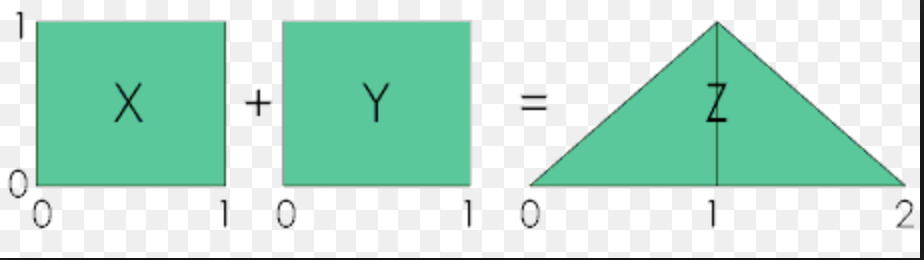
\includegraphics[scale = 0.8]{conv_u2.png}
\caption{The convolution of two uniform distributions $U[0,1]$.}
\end{figure}

This is actually why the distribution of dice rolls has a peak at $7$ and decreases in either direction, because it is the convolution of two uniform distributions (namely $U[1,6]$). 

In the discrete case, this is just 
\[ \PP(Z=k) = \sum_m \PP(X=m)\PP(Y=k-m).\] 

\subsection{Moment Generating Functions (Transforms)}
Recall from calculus that the exponential function has the series expansion 
\[ e^{sX} = 1 + sX + \dfrac{s^2}{2!}X^2 + \dfrac{s^3}{3!}X^3 + \dots.\] 
We can let $X$ be a RV. Then we can take expectation of both sides and apply linearity of expectation to get 
\[ M_X(s) = \EE[e^{sX}] = 1 + s\EE[X] + \dfrac{s^2}{2!}\EE[X^2] + \dfrac{s^3}{3!}\EE[X^3] + \dots .\] 

We call $M_X(s)$ the \textbf{moment generating function}, or \textbf{transform}, of $X$, for the following reason. All of the moments, i.e. RVs of the form $X^k$, are on the right hand side, and we can sift out whichever moment we need with a cute trick. If we want $\EE[X]$, then we can differentiate both sides with respect to $s$ and set $s = 0$, killing all the terms but $\EE[X]$. In symbols, 
\[ \dfrac{d}{ds}[M_X(s)] = \EE[X] + s\EE[X^2] + \dfrac{s^2}{2!}\EE[X^3] + \dots \] 
If we wanted $\EE[X^2]$, we can just take another derivative to get 
\[ \dfrac{d^2}{ds^2}[M_X(s)] = \EE[X^2] + s\EE[X^3] + \dots\] 
and set $s = 0$. In general, if we take $n$ derivatives, we find 
\[ \dfrac{d^n}{ds^n}[M_X(s)] = \EE[X^n] + s\EE[X^{n+1}] + \dots \]
from which setting $s$ to $0$ gives us the $n$th moment. 

What are the advantages of MGFs? 
\begin{enumerate}
    \ii Much easier to find the \emph{moments} of $X$. 
    \ii Much easier to \emph{multiply} than \emph{convolve}
    \ii Great analytical tool for proving things (CLT).
\end{enumerate}

Here's some properties. 
\begin{theorem}
    The moment generating function $M_X(s)$ of a RV $X$ satisfies the following properties. 
    \begin{enumerate}[(1)]
        \ii $M_X(0) = 1$. 
        \ii For $Y = aX + b$, $M_Y(s) = e^{sb}M_X(as)$.
    \end{enumerate}
\end{theorem}
\begin{proof}
    Part (a) is obvious. (Hint: use the very deep fact that $1 + 0 = 1$.)

    For part (b), just do the math. You get 
    \begin{align*}
        M_Y(s) &= \EE[e^{sY}] 
               = \EE[e^{s(aX+b)}] 
               = e^{sb}\EE[e^{asX}] = e^{sb} M_X(as).
    \end{align*}
\end{proof}

Let's get our hands dirty and find the MGFs of some common distributions. 
\begin{example}[Exponential MGF]
    Suppose we have a RV $X\sim \Expo(\la)$ which has pdf $f_X(x) = \la e^{-\la x}$ for $x\geq 0$. Then 
    \[ \EE[e^{sX}] = \int_0^{\infty} e^{sx}f_X(x) dx = \la\int_0^{\infty} e^{-\la x} e^{sx} dx = \la \dfrac{e^{-(\la-s)x}}{-(\la-s)} \Big|^{\infty}_0 = \dfrac{\la}{\la-s}\] 
    where $s < \la$ must hold in order for the integral to converge. Using this we can get $\EE[X] = M_X'(0) = \dfrac{\la}{(\la-s)^2}\Big|_{s=0} = \dfrac{1}{\la}$, and $\EE[X^2] = M_X''(0) = \dfrac{2}{\la}.$ 
\end{example}

\begin{example}[Poisson MGF]
    Now lets do the same for the Poisson distribution. Let $X\sim \Poisson(\la)$, so that $\PP(X=k) = \dfrac{e^{-\la}\la^k}{k!}$ for $k\geq 0$. Then 
    \[ M_X(s) = \EE[e^{sX}] = \sum_{k = 0}^\infty e^{sk}\dfrac{e^{-\la}\la^k}{k!} = e^{-\la}\sum_{k=0}^\infty \dfrac{(\la e^s)^k}{k!} = e^{-\la+\la e^s}.\]
    From this we can calculate $M_X'(0) = \la$ and $M_X''(0) = \la^2+\la$. 
\end{example}

\begin{example}[Normal MGF]
    Finally lets try the same for the normal distribution. Let $X\sim \Nor(0,1)$ so that $f_X(x) = \dfrac{1}{\sqrt{2\pi}}e^{-x^2/2}$. Then 
    \[ M_X(s) = \EE[e^{sX}] = \int_{-\infty}^\infty\dfrac{1}{\sqrt{2\pi}}e^{-x^2/2}e^{sx}dx.\]
    Now we're going to do a little bit of magic. The inside of this integral is $\exp(-x^2/2 + sx)$ which is a quadratic in $x$, so we're going to \emph{complete the square}. Hence, we get 
    \[ \dfrac{1}{\sqrt{2\pi}} \int_{-\infty}^\infty  \exp\left(-\dfrac{x^2-2xs+s^2}{2}\right) e^{s^2/2}dx = e^{s^2/2} \left[ \dfrac{1}{\sqrt{2\pi}} \int_{-\infty}^\infty e^{-(x-s)^2/2}dx\right].\]
    But the bracketed term is precisely our pdf integrated over its domain, which we already know to be 1. Hence, $M_X(s) = e^{s^2/2}$. This is super important, so know it. 

    If $Y\sim \Nor(\mu, \sigma^2)$, then $M_Y(s) = e^{s\mu}M_X(\sigma s)$, so $M_Y(s) = e^{s\mu}e^{\sigma^2s^2/2}$ is the MGF for general normal distributions. 
    
    It is left as an exercise to verifty that $M_X'(0) = 0$ and $M_X''(0) = 1$. 
\end{example}

\subsection{Inversions of transforms} 
Turns out $M_X(s)$ contains all of the info in $f_X(x)$ (under the mild condition that the moments are finite). This is known as the bilateral Laplace transform of $f_X(x)$. We can do inversions of these transforms using ``pattern matching,'' which is really just educating guessing lol. 

\begin{example}
    Suppose we have an MGF of $M_X(s) = \dfrac{1}{2}e^{-3s} + \dfrac{1}{4}e^{200s} + \dfrac{1}{4}e^s$. Recall that in the discrete case, transforms are a sum of terms of the form $e^{sx}$, so by comparing with the general formula 
  
    \[ M_X(s) = \sum_x e^{sx} p_X(x), \]

    we can recover our pdf as 
    \[ P(X = k) = \begin{cases}  
                    1/2 \quad \text{ when } k = -3 \\ 
                    1/4 \quad \text{ when } k = 200 \\ 
                    1/4 \quad \text{ when } k = 1 
            \end{cases} \] 
\end{example}

Here's the capstone on why we care so much about MGFs: we don't have to work with convolutions if we use them! Suppose we have $Z = X+Y$, where $X,Y$ are independent RVs. Then 
\[ M_Z(s) = \EE[e^{s(X+Y)}] = \EE[e^{sX}e^{sY}] = \EE[e^{sX}]\EE[e^{sY}],\]
avoiding any use of convolutions whatsoever! In summary, the MGF of the sum of two RVs is the product of their MGFs.

A quick application before we close out the day. Suppose $X\sim\Nor(\mu_X, \sigma_X^2)$ and $Y\sim\Nor(\mu_Y, \mu_Y^2)$. Then 
\[ M_Z(s) = M_X(s)M_Y(s) = \exp\left( \left(\dfrac{\sigma_X^2+\sigma_Y^2}{2}\right)s^2 + (\mu_X + \mu_Y)s \right) = MGF(\Nor(\mu_X+\mu_Y, \sigma_X^2+\sigma_Y^2)).\] 

\newpage
\section{Thursday, February 14th}
Happy Valentine's day to all the non-CS majors out there. As for the rest of you... 

\subsection{Moment Generating Functions (Review)}
The moment generating function of a random variable $X$ is $M_X(s) = \EE[e^{sx}]$, named as such because we can recover all of the moments $\EE[X^n]$ by taking derivatives. A quick result of this is that 
\[ \EE\left[\exp\left(s\sum_{i=1}^n X_i\right)\right] = \prod_{i=1}^n \EE[e^{sX_i}].\]

\subsection{Law of Total Variance}
 
\begin{theorem}[Total Variance]
    For random variables $X$ and $Y$, 
    \[ \Var(X) = \Var(\EE[X|Y]) + \EE[\Var(X|Y)].\] 
\end{theorem}
\begin{proof}
We expand intelligently; 
\begin{align*}
    \Var(X) &= \EE[(X-\EE[X])^2] \\ 
            &= \EE[(X - \EE[X|Y] + \EE[X|Y] - \EE[X])^2] \\ 
            &= \EE[(X-\EE[X|Y])^2] + 2\EE[(X-\EE[X|Y])(\EE[X|Y]-\EE[X])] + \EE[(\EE[X|Y] - \EE[X])^2] 
\end{align*}
where the last step was performed by grouping the first two terms and the last two terms and expanding. ``It is left as an exercise to show the middle term goes to 0,'' so we will focus on what we get from the remaining two terms. 

We will make use of the following fact. 

\begin{theorem}[Iterated Expectation]
    For random variables $X$ and $Y$, 
    \[ \EE[{\color{red}X}] = \EE[\EE[{\color{red}X} | {\color{blue}Y}].\] 
\end{theorem}

You can think of this as conditional expectation; we condition on $Y$ and find the expectation on the inside, and then ``sum out'' over all values of $Y$ by taking an expectation on the outside. Hence, we can rewrite 
\begin{align*}
    \EE[{\color{red}(X-\EE[X|Y])^2}] &= \EE[\EE[{\color{red}(X-\EE[X|Y])^2} | {\color{blue}Y}]] = \Var(\EE[X|Y]) \\
\EE[(\EE[X|Y] - \EE[{\color{red}X}])^2] &= \EE[(\EE[X|Y] - \EE[\EE[{\color{red}X}|{\color{blue}Y}]])^2] = \EE[\Var(X|Y)]
\end{align*}
from which our result follows 
\end{proof}

Here's an application as a quick reality check. \footnote{Thanks to Efe for the Piazza explanation.}

\begin{example}
    A chocolate store receives $B\sim \Bin(n,p)$ types of chocolate. When you go to the store, for each type of chocolate in the store, you toss an independent coin which has a probability $q$ of success. In summary, the amount of chocolate you buy is $C = \sum_{i = 1}^B \one_i$ where $\one_i$ is a Bernoulli RV with probability $q$. 

    We can compute the variance of $C$ using the law of total variance, which tells us that 
    \[ \Var(C) = \Var(\EE[C|B]) + \EE[\Var(C|B)].\] 
    
    First, notice that $C|B$ is a RV according to $\Bin(B, q)$; there are $B$ chocolates, and we have a probability $q$ of buying each one. Then $\EE[C|B]$ is $Bq$ by linearity of expectation, so 
    \[ \Var(Bq) = q^2\Var(B) = q^2np(1-p).\] 
    Also, $\Var(C|B)$ is $Bq(1-q)$, so 
    \[ \EE[Bq(1-q)] = q(1-q)\EE[B] = npq(1-q).\] 
    Putting it all together gives 
    \[ \Var(C) = npq^2(1-p) + npq(1-q) = npq(q-pq + 1-q) = npq(1-pq),\]
    which is precisely the variance of $\Bin(B, pq)$! This shouldn't be surprising, since we expected that the total number of things compounds in this way. 
\end{example}

\subsection{Tail Bounds}
This consists of a lot of CS 70 material (Markov's, Chebyshev's), but also some new bounds (namely the Chernoff bound). 

\begin{theorem}[Markov's Inequality]
    For a nonnegative random variable $X$, 
    \[ \PP(X \geq t) \leq \dfrac{\EE[X]}{t}\] 
    for all $t > 0$. 
\end{theorem}

This is important because tail bounds help us bound rare things that are away from the expectation. Think of a statistician who wants to bound the probability of errors in his/her data
% Insert picture of markov's on a normal distribution
\begin{proof}
    We condition on values of $X$, so 
    \begin{align*}
        \EE[X] &= \EE[X | X \leq t] \PP(X\leq t) + \EE[X | X \geq t]\PP(X\geq t) \\ 
               &\geq 0 + t \PP(X\geq t)
    \end{align*}
    where we can lower bound by $0$ since $X$ is nonnegative and we can lowerbound $\EE[X|X\geq t]$ by $t$ since we're conditioning on $X\geq t$. 
\end{proof}

The proof in our book uses coupling, which is creating a new random variable which is $0$ when $X\leq t$ and exactly $t$ when $X\geq t$, which leads to a similar proof as shown here. 

Let's try applying Markov's inequality to an exponential distribution $X\sim \Expo(\la)$. We have $\PP(X\geq t) = e^{-\la t}$ by the CDF, while Markov's inequality gives a bound of $\frac{1}{\la t}$, which is much looser. This might lead one to think that Markov's inequality is weak, but if all you know about a distribution is its mean, Markov's inequality is actually \emph{tight}! For a fixed $t$, there are distributions for which equality holds.

Of course, if you know more information you can obtain a better bound. Namely, 

\begin{theorem}[Chebyshev]
    For a random variable $X$, 
    \[ \PP(|X-\EE[X]| \geq t) \leq \dfrac{\Var(X)}{t^2}\] 
    for $t>0$.
    \label{thm:chebyshev}
\end{theorem}
\begin{proof}
    Using the very deep fact that $|a| > b \implies a^2 > b^2$, we find that 
    \[ \PP(|X-\EE[X]|\geq t) = \PP((X-\EE[X])^2 \geq t^2) \leq \dfrac{\EE[(X-\EE[X])^2]}{t^2} = \dfrac{\Var(X)}{t^2}\]
    where we can use Markov's inequality since $(X-\EE[X])^2$ is nonnegative. 
\end{proof}

\begin{example}
    Let $X\sim \Bin(n,p)$. By Markov, 
    \[ \PP(|X-\EE[X]|\geq t) \leq \dfrac{\EE[|X -\EE[X]|]}{t} \leq \dfrac{\EE[|X|+|\EE[X]|]}{t} = \dfrac{2\EE[X]}{t} = \dfrac{2np}{t}\] 
    where we used the triangle inequality to deduce that $|X-\EE[X]| \leq |X| + \EE[X]$ (triangle inequality is $|a+b| < |a| + |b|$), and $\EE[\EE[X]] = \EE[X]$ since expectation of a constant is a constant. 
    
    If we use Chebyshev, we get a bound of 
    \[ \PP(|X-\EE[X]|\geq t) \leq \dfrac{\Var(x)}{t^2} = \dfrac{np(1-p)}{t^2}\] 
    which is a factor of $t$ tighter than Markov. 
\end{example}

Before we go into Chernoff bounds, let's try to motivate them and see why they are interesting. Let's try bounding the probability $\PP(X\geq t)$ by the moments. By Markov, we have 
\[ \PP(f(X) \geq f(t)) \leq \dfrac{\EE[f(X)]}{f(t)}\] 
for $f(X) \geq 0$ and for all $f(t) > 0$. Hence, we can see that 
\[ \PP(X \geq t) \leq \dfrac{\EE[f(X)]}{f(t)}\] 
provided that $\PP(X\geq t) \leq \PP(f(X) \geq f(t))$; this can be achieved if $f$ is monotonically increasing, but this is merely sufficient, not necessary. 

Using this derived bound, we can bound probabilities by moments of our random variable by taking $f(t) = t^n$ to get  
    \[ \PP(X \geq t) \leq \dfrac{\EE[X^n]}{t^n}\] 
for $X\geq 0$, which is pretty good. The Chernoff bound is similar, offering us a bound in terms of the moments. 

\begin{theorem}[Chernoff Bound]
    For a random variable $X$, 
    \[ \PP(X\geq t) \leq \dfrac{\EE[e^{\la X}]}{e^{\la t}}\]
    for all $t$ and $\la > 0$.
\end{theorem}
\begin{proof}
    This should be second nature at this point. . Since $\la > 0$, 
    \[ \PP(X\geq t) = \PP(\la X \geq \la t) = \PP(e^{\la X} \geq e^{\la t}) \leq \dfrac{\EE[e^{\la X}]}{e^{\la t}}.\] 
\end{proof}

Important question of the day: why do we even need a $\la$ at all? 

Answer: Like the French revolution, it gives you freedom! (over how sharp of a bound you get). One thinks of it as a knob that you can adjust to give you a better (or worse) bound. Note that higher $\la$ isn't always better. 

Another note is that Chernoff bounds aren't always the best; if you have a Chernoff bound with a fixed $\la$, I can always come up with a better moment bound. 

\begin{example}
    Let's apply the Chernoff bound to normal random variables. We find that 
\[ \PP(X\geq t) \leq \dfrac{\EE[e^{-\la X}]}{e^{\la t}} = \dfrac{e^{-k^2\si^2/2}}{e^{\la t}}\] 
for $X\sim \Nor(0, \si^2)$. We want to pick the $\la$ that minimizes this, so we'll take logs and then differentiatie, because 
\[ \arg\min_\la \dfrac{e^{-k^2\si^2/2}}{e^{\la t}} = \arg\min_\la \dfrac{\la^2\si^2}{2} - \la t.\] 
    Differentiating this gives a solution $\la  = t/\si^2$, which gives a bound of $\PP(X\geq t) \leq e^{-t^2/2\si^2}$, which is literally as tight as possible since it's our CDF. Magic. 
\end{example}

\newpage
\section{Thursday, February 21st}
\subsection{Announcements}
HW 5 due next Wednesday. Reading is B\&T 5.2-5.6, Walrand 2.1-2.3. Apparently Chapter 2 is quite difficult to read, so proceed with caution. %Today is a lot of concentration variables.

\subsection{Weak and Strong Law of Large Numbers (Modes of Convergence)}
The idea of the weak law of large numbers is to look at the behavior of say coin flips in the long run. There's two questions we can start off our discussion with: how many heads (mean) will we get, and how variable are our results (variance)? 

We can describe it formally as such. We perform an experiment $n$ times independently and note 
\[ M_n = \dfrac{1}{n}\sum_{i=1}^n X_i \quad (X_i's \text{ i.i.d. })\] 
where $X_i$ has mean $\mu$ and variance $\sigma^2$. Then 
\[ \EE[M_n] = \EE\left[\dfrac{1}{n}\sum_{i=1}^n X_i\right] = \dfrac{1}{n} \EE[X_1]\cdot n = \EE[X_1] = \mu,\] 
and 
\[ \Var(M_n) = \dfrac{1}{n^2}\sum_{i = 1}^n \Var(X_i) = \dfrac{\si^2}{n}\] 
since the $X_i$ are i.i.d. If we take $n\to\infty$ to look at the long term behavior, $\EE[M_n] = \mu$ and $\Var(M_n) = 0$. 

This is cool and all, but wouldn't it be dope if we also knew the \emph{rate} at which the variance decreased to 0? We can do this by using Chebyshev (Theorem~\ref{thm:chebyshev}) to do a tail bound:
    \[ \PP(|M_n-\mu| > \epsilon) \leq \dfrac{\si^2}{n\epsilon^2},\]
     and just like that we've derived the weak law of large numbers. 
\begin{theorem}[Weak LLN]
    Suppose $X_1, X_2, \dots, X_n$ are i.i.d. RVs with mean $\mu$. Then for any $\epsilon > 0$, 
\[ \PP\left(\left|\dfrac{X_1+X_2+\dots + X_n}{n}-\mu\right| \geq \epsilon\right) \to 0 \]
    as $n\to\infty$. 
\end{theorem}

What does the Weak LLN really mean? In one way, it means that $\lim_{n\to\infty}\PP(|M_n-\mu|\geq \epsilon) = 0$. Now recall delta-epsilon limits from calculus: for any $\epsilon, \delta > 0$, there exists $n(\epsilon, \delta)$ (meaning $n$ is a function of $\epsilon,\delta$), large enough such that 
    \[ \PP(|M_n-\mu|\geq\epsilon) \leq \delta\] 
for $n> n(\epsilon, \delta).$ We can think of these variables as representing the following: 
\begin{align*}
    \epsilon &: \text{ ``accuracy level'' or error } \\ 
    \delta &: \text{ confidence level } \\ 
    n(\epsilon, \delta) &: \text{ threshold for a given accuracy/confidence } 
\end{align*}

Motivated by our above findings, we make an important definition: 

\begin{definition}
    We say a sequence of random variables $(M_n)_{n=1}^\infty = M_1, M_2, \dots$ \textbf{converges in probability} if for any $\epsilon > 0$, $\PP(|M_n-\mu| \geq \epsilon)\to\infty$ as $n\to\infty$, and denote it as $M_n\cinprob \mu$. 
\end{definition}

This gives us a notion of convergence for random variables/distributions, much like convergence of functions from Calculus.\footnote{Remember $\delta - \epsilon$ limits? yea those disgusting things.}

\begin{example}
    Suppose $X_1, X_2, \dots, X_n \sim U[-1, 1]$ are i.i.d., and $Y_n = \frac{X_n}{n}$. Then to find the density, we first find that 
    \[ Y_n \leq y \implies X_n \leq ny,\]
    so 
    \[ F_{Y_n}(y) = F_X(ny) \implies f_{Y_n}(y) = n f_X(ny). \] 
    %%%%%%%%%%% INSERT GRAPH %%%%%%%%%%%%%%
    If we plot $f_{Y_n}(y)$, it would be a rectangle with endpoints at $y = -1/n$ and $y = 1/n$ with height $n/2$ since $f_{Y_n}(y) = n/2$ for all $y$ in its domain. Then $\PP(|Y_n| \geq \epsilon) = 0$ if $n > \frac{1}{\epsilon}$, which is what it means to converge in probability. 
\end{example}

\begin{example}
    Let $Y_n = \min(X_1, X_2, \dots, X_n)$ where $X_i$'s are i.i.d. in $U[0,1]$. Then 
    \[ \PP(|Y_n - 0| \geq \epsilon) = \PP(X_1\geq \epsilon, X_2\geq \epsilon, \dots, X_n > \epsilon) = (1-\epsilon)^n \xrightarrow[n\to\infty]{\PP} 0 .\] 
    In other words, the probability that the minimum is greater than any $\epsilon$ you pick in the long run is $0$, which makes sense. 
\end{example}

\begin{example}
    Suppose time is in discrete units\footnote{``Bold move.'' - Phil} $(1, 2, \dots )$ and $Y_n = 1$ if there is an arrival at time $n$, $Y_n = 0$ otherwise. Define $I_k = \{2^k, 2^k+1, \dots, 2^{k+1}-1\}$, so that every next interval is twice as large as the next one. 
    %%%%%%%%%%%%%%%%%%%%%%%%%%%%%%%%%%%%%%%%%%%
    %
    %-----------------------------------------
    % 1 2 3 4 5 6 7 8 9 ...  15 16 
    %I0  I1 |--I2--| |---I3---|
    %
    %%%%%%%%%%%%%%%%%%%%%%%%%%%%%%%%%%%%%%%%%%%
    Suppose there is exactly $1$ arrival in each interval (equally likely). Then 
    \begin{align*}
        \PP(Y_1 = 1) &= 1 \\ 
        \PP(Y_2 = 1) = \PP(Y_3 = 1) &= \dfrac{1}{2} \\ 
                                    &\dots \\ 
        \PP(Y_n = 1) &= \dfrac{1}{2^k} \text{ if } n \in I_k.
    \end{align*}
    
    So $\lim_{n\to\infty}\PP(Y_n = 1) = \lim_{k\to\infty}\frac{1}{2^k} = 0$, meaning that $\PP(Y_n=1)$ converges to $0$ in probability. 
    
    This should be confusing however! Given any finite $n$, there are certain to be an infinite number of arrivals after $n$. Hence, we know for a \emph{fact} that $\PP(Y_n=1)$ will be nonzero infinitely often. 
    
    This example demonstrates the weakness of the weak LLN, and tells us that perhaps there are stronger notions of convergence than just convergence in probability. 
\end{example}

Before I state Strong LLN, I will first state what this stronger notion of convergence is. 

\begin{definition}
    Let $(M_n)_{n\geq 1}$ be a sequence of random variables. Then we say that $M_n$ converges \textbf{almost surely} to $\mu$ if 
    \[ \PP\left(\lim_{n\to\infty} M_n = \mu\right) = 1\] 
    and denote it by $M_n\asure \mu$. 
\end{definition}

\begin{theorem}[Strong LLN]
    Let $(X_n)_{n\geq 1}$ be a sequence of i.i.d. RV's with mean $\mu$. Then, 
    \[ \dfrac{1}{n}\sum_{i=1}^n X_i \to \mu \] 
    as $n\to\infty$ with probability $1$. In other words, if we let $M_n = \frac{1}{n}\sum X_i$, then $M_n\asure \mu$. 
\end{theorem}

\begin{proof}
    Walrand Chapter 2, but only for the brave. 
\end{proof}

Let's illustrate the difference between the Weak and Strong LLN with an example of rolling 6-sided die. The Strong LLN states that \emph{every} realization converges to $\mu$. So if we were to draw a plot of all different realizations, the Strong LLN states that all of them tend towards the line $X = \mu$. 

On the other hand, the Weak LLN only places a bounding box of width $2\epsilon$ around our mean, and says that the probability of any realizations outside this box is 0 in the long run. It doesn't say anything about occurences within the box, which is why our wacky example from above technically converges in probability. Hence, all we are guaranteed is that the \emph{fraction} of realizations outside $\mu\pm \epsilon$ for all $\epsilon, \delta > 0$ converges to $0$. 

\subsection{The Central Limit Theorem}

\begin{question}
    What happens to $S_n = \sum_{i = 1}^n X_i = X_1 + X_2 + \dots + X_n$ as $n\to\infty$?
\end{question}
\begin{proof}[Answer]
    You always end up with a normal distribution. Try it out for $X_i \sim U[0,1]$ or $X_i \sim \Exp(1)$ if you don't believe me. 
\end{proof}

    If we look at the variance and mean of $S_n\to \infty$ as $n\to\infty$, then we find that $\EE[S_n] = n\mu$ and $\Var(S_n) = n\si^2$. Hence we should normalize by defining 
\[ Z_n = \dfrac{S_n - n\mu}{\sqrt{n}\si}.\] 
You can check that this now has 0 mean and variance 1. Amazingly, this holds in general, which is what the CLT states. 

\begin{theorem}[Central Limit Theorem]
    Suppose $S_n = \sum_{i=1}^n X_i$ where the $X_i$ are i.i.d. RVs with mean $\mu$ and variance $\si^2$, and define $Z_n$ as above. Then, (amazingly), 
    \[ \lim_{n\to\infty} \PP(Z_n\leq x) = \Phi(x) \] 
    where $\Phi(x)$ is the c.d.f of the standard normal distribution $\Nor(0, 1)$. 
\end{theorem}

For large enough $n$, $Z_n\sim\Nor(0,1)$ in distribution, i.e. 
\begin{align*}
    S_n &\xrightarrow[n\to\infty]{d} \Nor(n\mu, n\si^2) \\
    Z_n &\xrightarrow[n\to\infty]{d} \Nor(0, 1) 
\end{align*}

where $\xrightarrow[n\to\infty]{d}$ is convergence in distribution, which we will not go into detail about. There are two implications. 
\begin{enumerate}
    \ii The distribution of $S_n$ and $Z_n$ ``wipe out'' all the information except for $\mu$ and $\si^2$. 
    \ii If there are a large number of small independent factors, the \emph{aggregate} of these factors will be normally distributed, which is just noise. 
\end{enumerate}

We end the day by outlining the proof of CLT. 
\begin{proof}[Proof of CLT]
    If $Y\sim \Nor(0,1)$, $M_Y(s) = \EE[e^{sY}] = e^{s^2/2}$. Then suppose $X_1, X_2, \dots, X_n$ are i.i.d. with mean $0$ and variance $1$ (WLOG). Let $M_X(s)$ be the MGF of each $X_i$, and let 
    \[ Z = \dfrac{X_1 + X_2 + \dots + X_n}{\sqrt{n}} \implies \EE[Z] = 0, \Var(Z) = 1.\] 
    Then 
    \[ M_Z(s) = \EE[e^{sZ}] = \EE[\exp(\frac{s}{\sqrt{n}}(X_1 + X-2 + \dots + X_n))].\] 
    We can finish the proof then by decomposing $M_Z(s)$ and using Taylor expansion. The rest of the proof will be discussed next week. 
\end{proof}

\newpage
\section{Tuesday, February 26th}
HW 5 is due tomorrow, and the readings are Walrand Ch 1, 2.4, 13.3, B\&T 6.1-6.4. 

\subsection{Wrapping up CLT}
From last lecture, suppose we have $S_n = \sum_{i=1}^n X_i$ where $X_i$ are i.i.d. with mean $\mu$ and variance $\si^2$. Then if let 
\[ Z_n = \dfrac{S_n - n\mu}{\sqrt{n}},\]
as $n\to\infty$, $Z_n$ has mean $0$ and variance $1$, giving us information about the long-term behavior of $S_n$. The Central Limit Theorem tells us more precisely that $\PP(Z_n\leq x) = \Phi(x)$ for every $x$. Let's prove CLT. 

\begin{proof}[Proof of CLT]
Let $X_1, X_2, \dots, X_n$ be i.i.d. with mean $0$ and variance $1$ and let $M_X(s)$ be the MGF of each of the $X_i$'s. Note that by definition, 
\[ Z = \dfrac{X_1 + X_2 + \dots + X_n}{\sqrt{n}} \implies \EE[Z] = 0, \Var(Z) = 1.\] 

Our goal is to be able to find the MGF of $Z$ as well. If we expand, we will get 
\begin{align*}
    M_Z(s) = \EE[e^{sZ}] &= \EE\left[e^{s\frac{1}{\sqrt{n}}(X_1 + X_2 + \dots + X_n)}\right] \\ 
                         &= \EE\left[e^{\frac{sX_1}{\sqrt{n}}}\right] \EE\left[e^{\frac{sX_2}{\sqrt{n}}}\right]\dots  \EE\left[e^{\frac{sX_n}{\sqrt{n}}}\right] \\ 
                         &= \EE\left[e^{\frac{sX_i}{\sqrt{n}}}\right]^n = \left[M_X\left(\frac{s}{\sqrt{n}}\right)\right]^n 
\end{align*}

Now recall Taylor's theorem: any infinitely differentiable function can be written as $f(x) = f(a) + f'(a)(x-a) + \dots + f^{(n)}(a)(x-a)^n + \dots$ (the \emph{Taylor} Series). So, 
\begin{align*}
    M_X(s) &= M_X(0) + M_X'(0)s + M_X''(0)\dfrac{s^2}{2!} + M_X'''(0)\dfrac{s^3}{3!}+\dots\\ 
           &= 1 + \EE[X]s + \EE[X^2]\dfrac{s^2}{2} + \EE[X^3]\dfrac{s^3}{6}\dots \\ 
           &= 1 + \dfrac{1}{2}s^2 + \dfrac{s^3}{6}\EE[X^3] 
\end{align*}

where we used our earlier facts that $\EE[X] = 0$ and $\EE[X^2] = \Var(X)+\EE[X]^2 = 1$. Plugging this into our MGF for $Z$ gives 
\[ M_Z(s) = \left[M_X\left(\frac{s}{\sqrt{n}}\right)\right]^n = \left[1 + \dfrac{s^2}{2n} + \dfrac{s^3}{6n^{3/2}}\EE[X^3] + \dots \right]^n\]  
\[ \implies \lim_{n\to\infty} M_Z(s) = \lim_{n\to\infty} \left[ 1 + \dfrac{s^2}{2n} + \dfrac{s^3}{6n^{3/2}}\EE[X^3] + \dots \right]^n.\] 

This looks really similar to our classic limit of the form $\lim_{n\to\infty}(1+\frac{x}{n})^n = e^x$, but its got these higher order terms that we'd ideally like to ignore. Turns out that those terms actually don't matter; the only ones we care about are the first two. We write this as $o(\frac{1}{n})$ (little $o$ notation) to show that in the limit these terms disappear, so 
\[ \lim_{n\to\infty} M_Z(s) = \lim_{n\to\infty} = \left[1+\dfrac{s^2/2}{n} + o\left(\dfrac{1}{n}\right)\right]^n = e^{s^2/2} = M_Y(s)\] 
completing our proof. 
\end{proof}

Here's an application of CLT to testing light bulbs. 
\begin{example}
    Light bulbs have i.i.d $\Expo(\la)$ lifetimes. We want to make sure that $\frac{1}{\la} > 1$. Say we measure the average lifetimes $A_n$ of $n = 100$ bulbs and find $A_{100} = 1.2$. Then $A_n = \frac{1}{n}\sum_{i=1}^n S_i$, so 
    \begin{align*}
        \EE[A_n] &= \frac{1}{\la} \\ 
        \Var(A_n) &= \frac{1}{n^2}\cdot n \cdot \frac{1}{\la^2} = \frac{1}{n\la^2}. 
    \end{align*}
    \begin{question}
        What is the confidence that we have $\frac{1}{\la} > 1$? 
    \end{question}
    Let $Z_n = \dfrac{A_n - \frac{1}{\la}}{\frac{1}{\sqrt{n}}\la}$, so that $Z_n$ has $0$ mean and variance $1$. Then by CLT, $Z_n\sim \Nor(0,1)$. Taking $n = 100$ gives 
    \[ Z_{100}  = \dfrac{A_{100} - \frac{1}{\la}}{\frac{1}{10\la}} = 10(1.2\la -1) = 12\la - 10.\] 
    So to find our probability, we simply calculate 
    \[ \PP(\la < 1) = \PP(12\la - 10 < 2) = \PP(\Nor(0,1) < 2) = 97.5\%\] 
    Note this approximation is an asymptotic estimation and not a bound, but a damn good one at that. 
\end{example}

\subsection{Information Theory}
This entire field was born with Claude Shannon's 1948 paper \emph{A mathematical theory of communication}, which was actually rejected from the publishing journal Shannon sent it to for not being rigorous enough. The reviewer of the paper remarked 30 years later that, ``One of my biggest regrets was rejecting that paper.'' 


\begin{figure}[!ht]
    \centering
    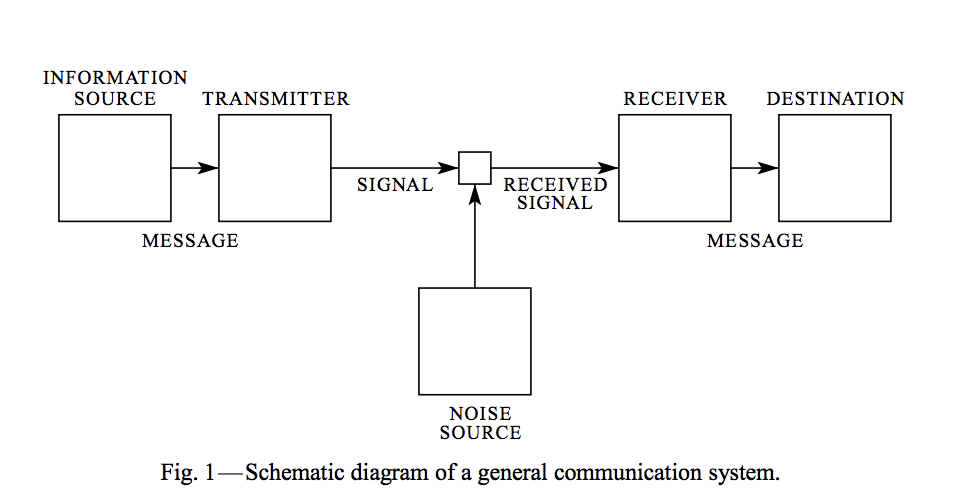
\includegraphics[scale=0.8]{shannon_paper_fig.png}
\caption{Shannon's proposed communication framework (Shannon 1948).}
\end{figure}

\begin{theorem}[Separation]
    There is no loss of optimality in separating source-coding (compression) from channel coding (reliable communication). 
\end{theorem}

\begin{example}[Source Coding]
    Let $X\sim\{0,1\}$ with $\PP(X=1) = p$, and let $X^{(n)} = \{010\dots\}$ be an $n$-length $\Ber(p)$ source. Suppose we have a file of length 10,000. and it was $\Ber(p)$ i.i.d. What is the compression limit?  

    The entropy $H(X)$ is 
    \[ H(X) = -\sum_{x\in\{0,1\}}p(x) \log p(x) = -p\log p - (1-p)\log(1-p) = h(p).\] 
    If we plot $h(p)$, we can see a parabola like shape with a maximum of $1$ at $p = 0.5$, so we can't compress it at all. If $p = 0.11$, then $h(p) = 0.5$ between symbols, so a 10,000 length file has a 5,000 length compression limit. 
\end{example}

If one is interested in more Information Theory, look into taking EE 229A. 

\subsection{Asymptotic Equipartition Property}
If I have an $n$-length $\Ber(p)$ sequence, we will have $np$ heads and $n(1-p)$ tails. Then AEP says that out of the $2^n$ total sequences, the number of sequences that I can expect to see, $\binom{n}{np}$, is approximately $2^{n h(p)}$ (using Stirling's apprx.), so each sequence appears with probability $2^{-n h(p)}$. 

We also talked about Binary Erasure Channels and their Capacities. Sorry I got really lazy and didn't bother taking notes about those. I'll add them back in once I get the time to. :) 

\newpage
\section{Thursday, February 28th}
HW 6 is released, due next Wednesday. Reading is Walrand Chapter 1, 13.3 and B\&T Chapters 7.1-7.4, plus the notes on BECs. 

\subsection{Capacity of the BEC}
The goal of today is to find the \emph{capacity} of the BEC$(p)$ channel. Capacity is the maximum rate of reliable communication, which we can define as 
\[ \text{ Rate } = \dfrac{ \text{\# of bits reliably sent}}{\text{\# of channel uses}} = \dfrac{L(n)}{n} \text{ bits/ch use}.\]

We also make the following definitions (which can be seen in the diagram): 

\[ f_n(\cdot) \text{ is the encoding function that maps } \{0,1\}^L\to\{0,1\}^n \] 
\[ g_n(\cdot) \text{ is the decoding function that maps } \{0,1, *\}^n\to\{0,1\}^L \] 

We can let $P_e^{(n)} = \max_{m=\{0,1\}^L} \PP(m\not= \hat{m})$ denote the probability of error. Let me explain why this makes sense. We take the max to get the ``worst case'' error, and we take $m = \{0,1\}^L$ as an approximation of sending many messages. Of course, the probability is precisely the event of an error, when our sent message is different from the decoded message.

Finally, let $R = L/n \text{ bits/channel use}$. We say that rate $R$ is \emph{achievable} for the channel if for every $n$, there exists encoding and decoding functions such that $P_e^{(n)} \xrightarrow[n\to\infty]{} 0$ (which exact mode of convergence is t.b.d.). The largest achievable rate $R$ is called the \textbf{capacity} of the channel, denoted $C_{\BEC{p}}$. 

Now the stage is set for us to state Shannon's theorem. 
\begin{theorem}[Shannon 1948]
    $C_{\BEC{p}} = 1-p$ bits per channel use. 
\end{theorem}

There are two statements hidden within this theorem. The capacity of the BEC is at most $1-p$, and that this maximum is also attainable. 

\begin{proof}
    We first show that the capacity cannot exceed $1-p$. Assume we have a friendly genie who relays instantaneously to the sender (TX) whenever the received symbol is a $*$. Then the best rate is to resend whichever symbols are erased. Hence, the time for a bit to get through the channel is approximately $\Geo(1-p)$, so the expected time it takes a bit to get through is $1/(1-p)$. Hence, $C \leq 1-p$ bits per channel use. 

    Now we do the forward direction to show this maximum is attainable. We'll show that $R = 1-p-\epsilon$ for all $\epsilon > 0$ is achievable. Shannon's insight was to leverage the Strong LLN. By Strong LLN, the probability of channel erases exactly $np$ symbols is $1$. In other words, as $n\to\infty$, $\PP(np\text{ bits erased})\to 1$. 

    Next we populate a lookup table of size $2^L$ by $n$ with i.i.d. $\Ber(1/2)$ entries. Call this table a \emph{codebook} $\mathcal{C}$, and allow it to be shared between the sender and the receiver before hand. 

    \begin{figure}[!ht]
\[
\begin{array}{C|C|C|C|C|C}
    & 1 & 2 & 3 & \dots & $n$ \\
\hline
1 & 1 & 1 & 0 & \dots & 1 \\
2 & 0 & 1 & 1 & \dots & 0 \\
3 & 1 & 0 & 1 & \dots & 0 \\
\vdots & \vdots & \vdots & \vdots & \ddots & \vdots \\
$2^L$ & 1 & 0 & 0 & \dots & 1 \\
\end{array}
\]
\caption{An example of a codebook $\mathcal{C}$.}
\end{figure}


    Suppose we transmit a message in the $i$th row of $\mathcal{C}$. On average, by SLLN, there are $np$ bits that are erased. WLOG assume they are at the end of the message. The receiver will drop the last $np$ columns of the codebook to obtain a truncated codebook $\mathcal{C}'$. Then he will follow these rules for decoding: 
    \begin{enumerate}
        \ii If $c_j'$ is the \emph{only} entry in $\mathcal{C}'$ matching $Y^{(n(1-p))}$ ($Y^n$ without the last $np$ bits), then decode $\hat{m} = j$. 
        \ii Else, declare ERROR. 
    \end{enumerate}
    If this sounds like a really dumb idea you're not wrong. But it turns out this is just enough for us to attain the maximum. To see this, we need to calculate the probability of an error.  
\begin{align*}
    \PP(\text{error}) = \PP(c'_i\text{ is not unique}) 
    &= \PP\left(\bigcup_{i\not= j} \{c_i' = c_j'\}\right) \\ 
    &= \sum_{i\not= j} 2^{-n(1-p)} < 2^L 2^{-n(1-p)}
\end{align*}
by the union bound. Hence, $P_e \leq 2^{n(R-(1-p))}$. In order for $P_e \xrightarrow[n\to\infty]{} 0$, we need $R-(1-p) < 0$, or $R < 1-p$. So we just make $R = 1-p-\epsilon$ so that $P_e \leq 2^{-n\epsilon} \xrightarrow[n\to\infty]{} 0$ for all $\epsilon > 0$. 
\end{proof}

Here's a quick engineering example with some numbers. 
\begin{example}
    Suppose we take $n = 10,000$, $p = 1/2$ and $\epsilon = 0.01$. Then 
    \[ C_{\BEC{\frac{1}{2}}} = \dfrac{1}{2} \text{ bits/ch. use } \implies C = 5000\text{ bits.}\] 
    So we set our $R$ to $1-\frac{1}{2} - 0.01 = 0.49$ which means $L = 4900$ bits. Hence $P_e \leq 2^{-n\epsilon} = 2^{-100} \approx 0$. This means that we can can send $4900$ with basically no errors. Neat. 
\end{example}

\subsection{Markov Chains}

We will often want to study stochastic processes $X = \{X_t\}_{t\in T}$, which are a collection of RVs, where the index $t$ often refers to a representation of time. $X$ models the evolution of a sequence of RVs as a function of time. Some examples are stock prices, your wealth, customers, etc. 

In general, to characterize the behavior of $X: (X_1, X_2, \dots, X_n)^\infty$, we would need the joint pdf of $X_1, X_2, \dots, X_n$. This is a \emph{bad idea}, since it will very quickly grow too large for any reasonable computation. Hence we impose some structure on the process and get a markov chain. 

\begin{definition}
    Let $\mathcal{X}$ be a finite set (called the state space) with random variables $X_i$ drawn from it. Then if 
    \[ \PP(X_n = x_n | X_{n-1} = x_{n-1}, \dots, X_1 = x_1) = \PP(X_n = x_n | X_{n-1} = x_{n-1}),\] 
    we call $X_n$ a \textbf{Markov Chain}.
\end{definition}
The above property is called the ``amnesia'' or Markov property, since your state today only depends on your state yesterday and so on. 

\begin{figure}[!ht]
\begin{center}
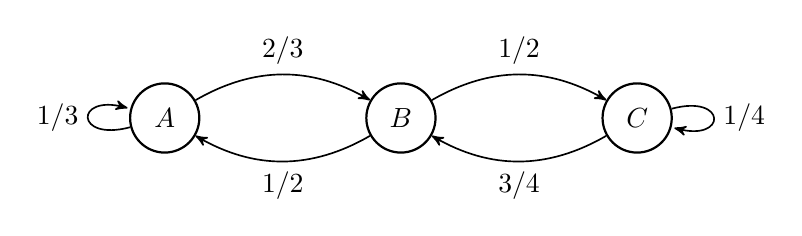
\begin{tikzpicture}[->, >=stealth', auto, semithick, node distance=3cm]
\tikzstyle{every state}=[fill=white,draw=black,thick,text=black,scale=1]
\node[state]    (A)                     {$A$};
\node[state]    (B)[right of=A]   {$B$};
\node[state]    (C)[right of=B]   {$C$};
\path
(A) edge[loop left]     node{$1/3$}         (A)
    edge[bend left, above]    node{$2/3$}      (B)
(B) edge[bend left, above]    node{$1/2$}           (C)
    edge[bend left, below]     node{$1/2$}           (A)
(C) edge[loop right]    node{$1/4$}           (C)
    edge[bend left, below]     node{$3/4$}           (B);
\end{tikzpicture}
\end{center}
\caption{An example of a Markov Chain}
\end{figure}
Based on the Markov Chain, you can also come up with its transition matrix, which is just a matrix that encodes the Markov property, $\PP(X_n | X_{n-1})$. 

\end{document}
